%\section{Validation du positionnement du module SEIS}
\section{Modélisation de la motorisation}
\begin{marginfigure}
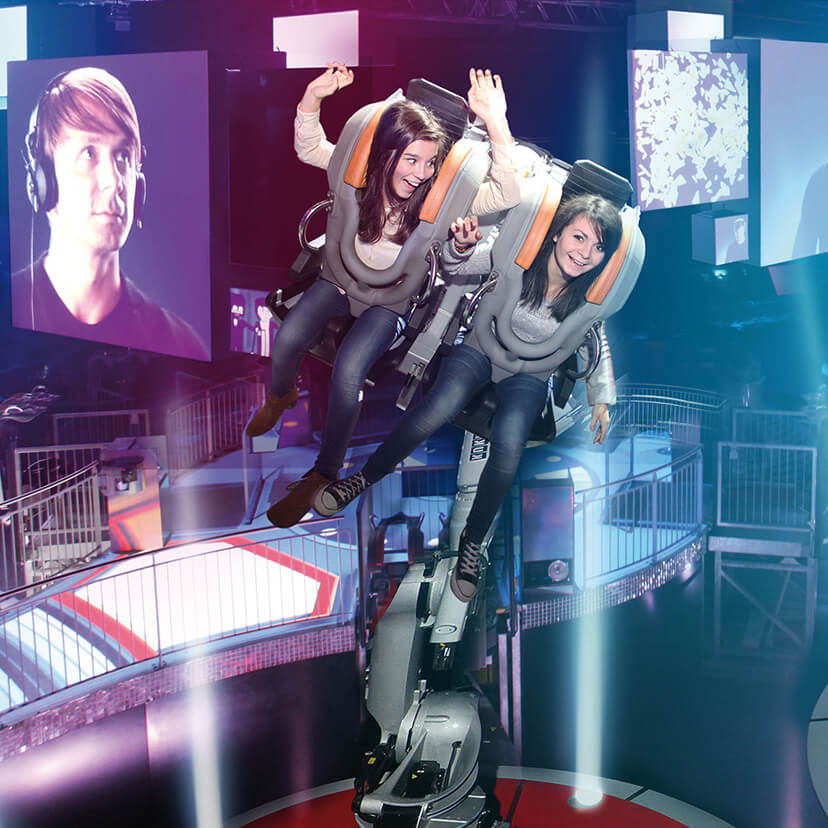
\includegraphics[width=\linewidth]{fig_01.jpg}
\caption{Sous-système SEIS \label{fig_01}}
\end{marginfigure}

\begin{obj}
Valider les réglages dela commande des trois actionneurs linéaires associés aux pieds, afin de respecter les exigences liées à leur positionnement.
\end{obj}

%
%
%On s'intéresse ici au sous-système SEIS. Il est basé sur un instrument
%hybride composé :
%\begin{itemize}
%\item d'un système de déploiement (DPL);
%\item d'une sphère comportant trois capteurs sismiques à très larges bandes et leurs capteurs de
%température;%. La sphère dispose d’un système de référencement de ses pieds (figure 3). Sa masse est d'environ \SI{3}{kg};
%\item d'une boîte électronique d'acquisition dont la structure est donnée par le diagramme de
%définition des blocs. 
%\end{itemize}



Afin d'être positionné, le SEIS est équipé de 3 pieds positionnés par des vérins électriques(aussi appelés actionneurs linéaires) asservis en position. Leur chaîne structurelle est donnée sur la figure \ref{fig_09}.

\begin{figure}[!h]
\centering
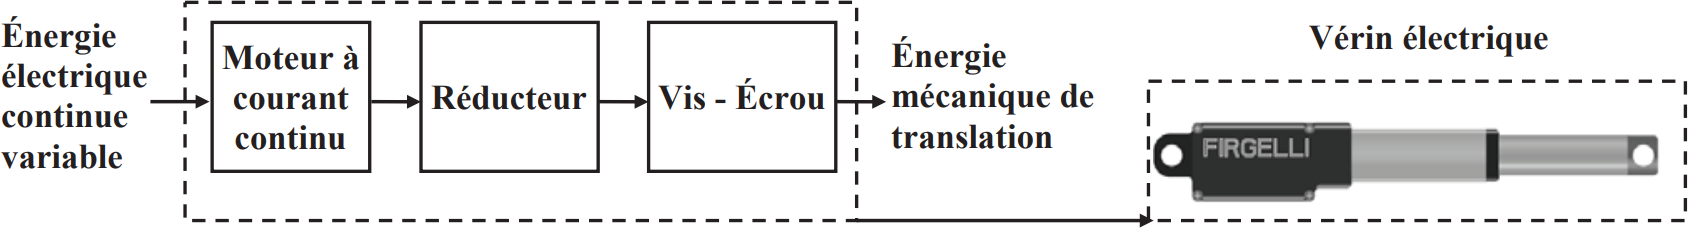
\includegraphics[width=\linewidth]{fig_09.png}
\caption{Chaîne structurelle de l’actionneur électrique linéaire \label{fig_09}}
\end{figure}


La table \ref{tab_01} dresse la liste des notations et spécifications. 

\begin{table*}[!h]
\begin{multicols}{3}
\begin{itemize}
\item masse à déplacer pour chaque vérin : $M =\SI{1}{kg}$;
\item pesanteur de la Terre : $g = \SI{9,81}{m.s^{-2}}$;
\item rapport de réduction du réducteur : $r = 0,01$;
\item rendement du réducteur : $\eta_r = 0,95$;
\item pas de la vis du système vis-écrou : $p = \SI{12}{mm}$;
\item rendement du système vis-écrou : $\eta_v = 0,96$;
\item coefficient de frottement visqueux du moteur : $f=\SI{0,002}{Nms/rad}$;
\item moment d’inertie équivalent total ramené sur l’arbre moteur : $J = \SI{0,00004}{kg.m^2}$;
\item résistance de l’induit de la MCC (Machine à Courant Continu) : $R =\SI{1}{\Omega}$;
\item inductance de l’induit de la MCC : $L = \SI{20}{\mu H}$;
\item constante de couple : $K_c = \SI{0,35}{NmA^{-1}}$;
\item constante de force contre électromotrice : $K_e = \SI{0,35}{Vs/rad}$;
\item tension d’alimentation de l’induit de la MCC : $u(t)$ en \si{V};
\item courant absorbé par l’induit de la MCC : $i(t)$ en \si{A};
\item vitesse de rotation en sortie de la MCC : $\omega(t)$ en \si{rad/s};
\item position angulaire en sortie de la MCC :  $\theta(t)$ en \si{rad};
\item force contre électromotrice de la MCC : $e(t)$ en \si{V};
\item couple moteur de la MCC : $C_m(t)$ en \si{Nm};
\item couple résistant total ramené sur l’arbre moteur : $C_r(t) = \dfrac{Mgpr}{2\pi \eta_v \eta_r} h(t)$\footnote{$h(t)$ désigne la fonction de Heaviside qui prend la valeur 0 pour t<0, 1 sinon.} en \si{Nm}.
\end{itemize}
\end{multicols}
\caption{Notations et spécifications \label{tab_01}}
\end{table*}

\textbf{Équations du moteur à courant continu :}
\begin{multicols}{2}
\begin{itemize}
\item équation électrique : $u(t)=e(t)+Ri(t)+L\dfrac{\dd i(t)}{\dd t}$;
\item équations de couplage électro-mécanique : $e(t)=K_e \omega(t)$, $C_m(t)=K_C i(t)$.
\end{itemize}
\end{multicols}


%
%La structure du schéma-bloc obtenue à partir du modèle de connaissance de la MCC est présentée sur la figure suivante.
%
%\begin{figure}[!h]
%\centering
%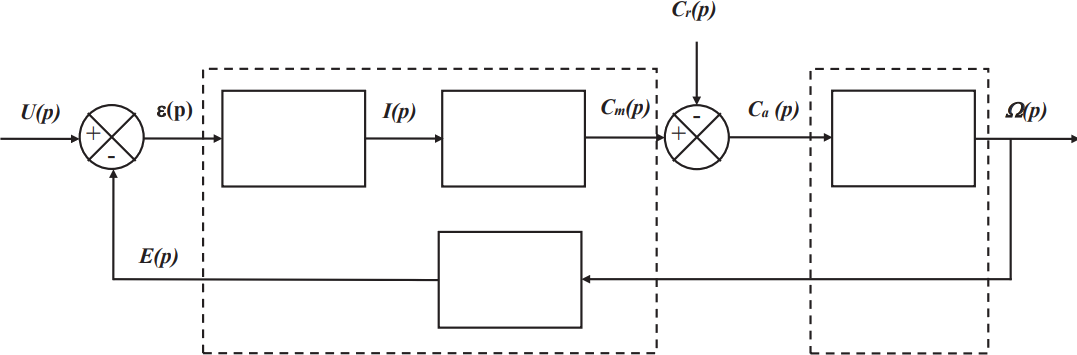
\includegraphics[width=\linewidth]{dr_01.png}
%\caption{Structure du schéma bloc \label{dr_01}}
%\end{figure}
%
%\question{À partir des équations du moteur à courant continu, compléter sous forme
%littérale les schémas bloc modélisant la MCC.}

L'application du théorème du moment dynamique à l'arbre moteur permet d'écrire l'équation suivante : 
$$
J\dfrac{\dd \omega(t)}{\dd t}  = C_m(t)-C_r(t)-f\omega(t).
$$

\question{Proposer un schéma-bloc du moteur à courant continu.}

On se place dans le cas particulier où $C_r(p) = 0$.

\question{Donner l’expression, sous sa forme canonique, de la fonction de transfert en boucle fermée $\indice{F}{m1}(p)=\dfrac{\Omega(p)}{U(p)}$.}


La figure \ref{dr_02} présente les résultats expérimentaux de l’évolution de la vitesse de rotation, $\omega(t)$ à la suite de l’application d’un échelon de tension $u(t)$ d’une amplitude de \SI{12}{V} aux bornes de la MCC. %On pose $\indice{F}{m2}(p)=\dfrac{\Omega(p)}{U(p)} = \dfrac{F_0}{1+T_0p}$

\begin{figure}[!h]
\centering
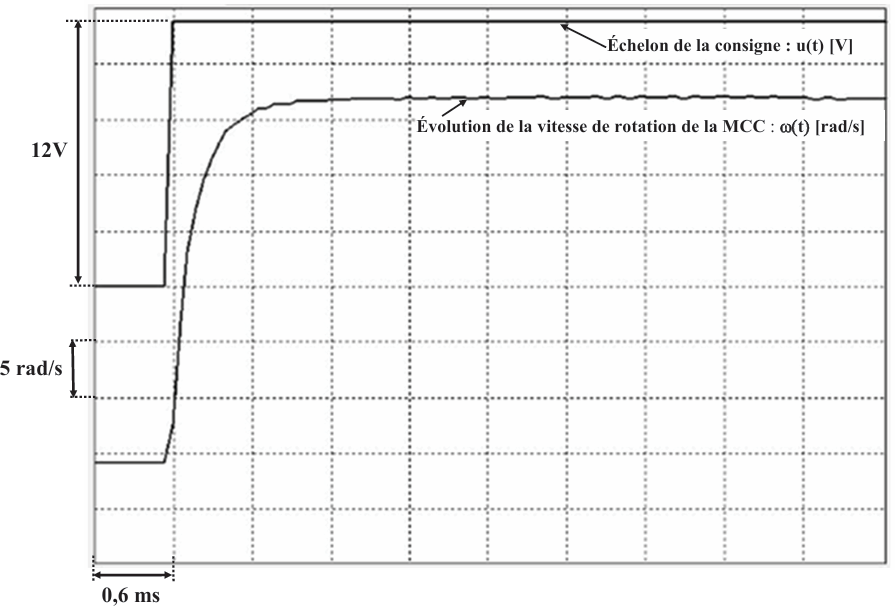
\includegraphics[width=.8\linewidth]{dr_02.png}
\caption{Réponse de la MCC à un échelon de \SI{12}{V}\label{dr_02}}
\end{figure}

% Q18
%\question{Justifier le choix d’une fonction de transfert d’ordre 1 pour modéliser le comportement de la MCC à partir des essais expérimentaux. Effectuer les constructions graphiques nécessaires sur la figure \ref{dr_02} afin de déterminer la valeur du gain statique $F_0$ et de la constante de temps $T_0$ de $\indice{F}{m2}(p)$. Proposer une hypothèse simplificatrice permettant de justifier le passage à l’ordre 1 de $\indice{F}{m2}(p)$ par rapport à $\indice{F}{m1}(p)$.}

\question{Proposer et justifier un modèle de comportement du moteur à courant continu $\indice{F}{m2}(p)$.}